\documentclass[red,10pt]{beamer}
%\setbeamertemplate{theorems}[numbered]
\usetheme{Warsaw}
\usecolortheme{default}
\usepackage{makeidx}
\usepackage[brazil]{babel}
\usepackage[utf8]{inputenc}
\usepackage[T1]{fontenc}
\graphicspath{{./figuras/}}             % caminho das figuras (recomendável)
\usepackage[noend]{algorithmic}
\usepackage{algorithm}
\usepackage{qtree}
\usepackage{graphicx}
\usepackage[caption=false]{subfig}
\uselanguage{portuguese}
\languagepath{portuguese}
\newtheorem{proposition}{Proposição}
\newtheorem{assertion}{Asserção}
\newtheorem{conjecture}{Conjectura}
\deftranslation[to=portuguese]{Theorem}{Teorema}
\deftranslation[to=portuguese]{Definition}{Definição}
\deftranslation[to=portuguese]{Fact}{Fato}
\deftranslation[to=portuguese]{Lemma}{Lema}
\usepackage{enumerate}
\algsetup{indent=2em}
\usepackage{tikz}
\usetikzlibrary{trees}
\algsetup{linenodelimiter=\ }
\floatname{algorithm}{Algoritmo}
\newcommand{\GL}{Gyárfás \& Lehel}

\title{Teoria dos Números e Computação: Uma abordagem utilizando problemas de competições de programação}
%\title{Teoria dos Números e Computação: Uma abordagem utilizando problemas de competições de programação}
\author{Antonio Roberto de Campos Junior \\ {Supervisor: Carlos Eduardo Ferreira } }
\institute{Instituto de Matemática e Estatística\\Universidade de São Paulo}
%\date{}

\begin{document}

\frame{\titlepage}
  
\frame{
	\frametitle{Agenda}
	\tableofcontents[ 
		currentsubsection, 
		hideothersubsections, 
		sectionstyle=show, 
		subsectionstyle=show,
		] 
}

\section{Introdução}

\frame{
	\frametitle{Objetivos}
	\begin{itemize}[<+->]
		\setlength{\itemsep}{5pt}
		\item Estudar tópicos específicos relacionados à Teoria dos Números
		\item Criar um material que mostre a aplicação direta dessa teoria na solução de problemas de competições de programação
		\item Demonstração da teoria e implementação dos algoritmos que resolvem os problemas que serão abordados
	\end{itemize}
}
\setcounter{subfigure}{0}


\frame{
	\frametitle{Motivação}
	\begin{itemize}[<+->]
		\setlength{\itemsep}{5pt}
		\item Experiência nesse tipo de competição
		\item Falta de um bom material didático nesse molde
	\end{itemize}
}
\setcounter{subfigure}{0}


\frame{
	\frametitle{A conjectura}
	\begin{conjecture}[{\GL}, 1976]
		Uma sequência de árvores $T_1,\ldots,T_n$ pode ser empacotada no~$K_n$.
	\end{conjecture}
	\vfill
	\begin{itemize}[<+->]
		\setlength{\itemsep}{8pt}
		\item Problema ainda em aberto.
		\item Técnicas usadas para encontrar respostas afirmativas.
		\vskip 5pt
		\begin{itemize}[<+->]
			\setlength{\itemsep}{5pt}
			\item Restringir as classes das árvores.
			\item Restringir o tamanho da sequência.
		\end{itemize}
	\end{itemize}
}

\section{Conjectura de {\GL}}

\subsection{Restringindo a classe das árvores}

\begin{frame}{\secname}
  \tableofcontents[currentsection,currentsubsection]
\end{frame}

\frame{
	\frametitle{Resultados conhecidos}
	\
	Quando restringimos as classes das árvores.
	\vskip 5pt
	\begin{itemize}[<+->]
		\setlength{\itemsep}{8pt}
		\item Sequências com no máximo 2 árvores diferentes de estrela. \\({\GL}, 1976) 
		\item Estrelas e caminhos. ({\GL} e Zaks \& Liu, 1976) 
		\item Subclasse de lagartas e aranhas. (Fishburn, 1983)
		\item Estrelas e biestrelas. (Hobbs et al., 1987)
		\item Quase-estrelas. (Dobson, 1997)
	\end{itemize}
}

\setcounter{subfigure}{0}

\frame{
	\frametitle{Estrelas}
	Dado um empacotamento de $T_1, \ldots, T_{n-1}$ no~$K_{n-1}$, como empacotar $T_n$?
	\pause
	\par 
	Adicionamos um novo vértice.
	\begin{figure}
  	\centering
  	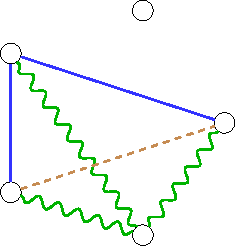
\includegraphics{stars1.pdf}
  	\caption{Empacotamento de $T_1,\ldots,T_4$ no $K_4$}
	\end{figure}
}

\setcounter{subfigure}{0}

\frame{
	\frametitle{Estrelas}
	Dado um empacotamento de $T_1, \ldots, T_{n-1}$ no~$K_{n-1}$, como empacotar $T_n$?
	\par
	
	Ligamos o novo vértice a $K_{n-1}$.
	\begin{figure}
  	\centering
  	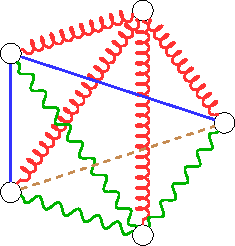
\includegraphics{stars2.pdf}
  	\caption{Empacotamento de $T_1,\ldots,T_5$ no $K_5$}
	\end{figure}

}

\setcounter{subfigure}{0}
	
\frame{
	\frametitle{Biestrelas}
	Dado um empacotamento de $T_1, \ldots, T_{n-1}$ no~$K_{n-1}$, como empacotar $T_n$?
	\pause
	\setcounter{subfigure}{0}
	\begin{figure}
  	\centering
  	\subfloat[$T_n$]{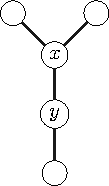
\includegraphics{bistar.pdf}}
	\qquad \qquad 
  	\subfloat[$K_{n-1}$]{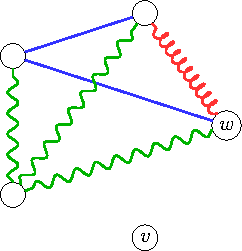
\includegraphics[scale=0.9]{bistar2.pdf}} 
	\end{figure}
	
}

\setcounter{subfigure}{0}

\frame{
	\frametitle{Biestrelas}
	Dado um empacotamento de $T_1, \ldots, T_{n-1}$ no~$K_{n-1}$, como empacotar $T_n$?
	\par
	Mapeamos $x$ em $w$
	\begin{figure}[h]
		\centering
  		\subfloat[$T_n$]{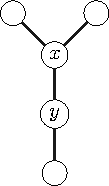
\includegraphics{bistar.pdf}}
		\qquad \qquad
		\subfloat[$K_{n-1}$]{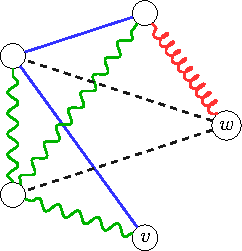
\includegraphics[scale=0.9]{bistar5.pdf}} 
	\end{figure}
}

\setcounter{subfigure}{0}

\frame{
	\frametitle{Biestrelas}
	Dado um empacotamento de $T_1, \ldots, T_{n-1}$ no~$K_{n-1}$, como empacotar $T_n$?
	\par
	Mapeamos $x$ em $w$ e $y$ em $v$.
	\begin{figure}[h]
		\centering
  		\subfloat[$T_n$]{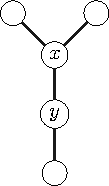
\includegraphics{bistar.pdf}}
		\qquad \qquad
		\subfloat[$K_n$]{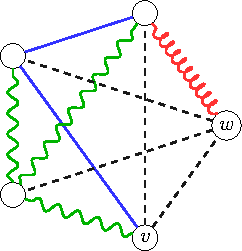
\includegraphics[scale=0.9]{bistar3.pdf}} 
	\end{figure}
}

\frame{
	\frametitle {Subclasse de lagartas e aranhas}
	\begin{itemize}
		\setlength{\itemsep}{8pt}
		\item $H_n$ grafo com sequência de graus $(n-1,\ldots,\lfloor n/2 \rfloor,\lfloor n/2 \rfloor, \ldots,1)$.
		\item $H_n$ e $H_{n-1}$ constituem uma decomposição do $K_n$.
	\end{itemize}
	\vfill
	\pause
	\setcounter{subfigure}{0}
	\begin{figure}[h]
		\centering
  		\subfloat[$H_6$]{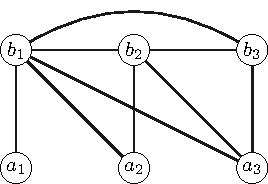
\includegraphics[scale=0.7]{H_6.pdf}}
		\qquad \qquad
		\subfloat[$H_5$]{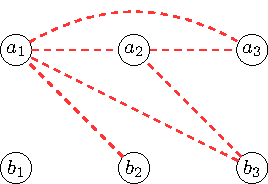
\includegraphics[scale=0.7]{H_5.pdf}} 
	\end{figure}
}

\frame{
	\frametitle {Subclasse de lagartas e aranhas}
	\begin{itemize}
		\setlength{\itemsep}{8pt}
		\item $H_n$ grafo com sequência de graus $(n,n-1,\ldots,\lfloor n/2 \rfloor,\lfloor n/2 \rfloor, \ldots,1)$.
		\item $H_n$ e $H_{n-1}$ constituem uma decomposição do $K_n$.
	\end{itemize}
	\vfill

	\begin{theorem}[Fishburn, 1983]
		$T_{n}$ e $H_{n-2}$  podem ser empacotados em $H_{n}$ se $T_{n}$ é uma estrela, ou
		uma biestrela, ou uma triestrela unimodal, ou um caminho, ou uma lagarta 3-interior ou um escorpião.  
	\end{theorem}
	\vfill
	\textbf{Ideia:} Se $n$ par, empacotar $T_2, T_4 , \ldots, T_n$ em $H_n$, e $T_1, T_3, \ldots , T_{n-1}$
	em $H_{n-1}$.
}

\setcounter{subfigure}{0}

\frame{
	\frametitle{Caminhos}
	Se $T_n$ é um camino, como empacotar $T_n$ em $H_n$?
	\pause
	\setcounter{subfigure}{0}
	\begin{figure}
		\centering
  		\subfloat[$H_6$]{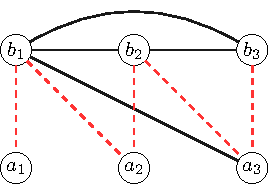
\includegraphics[scale=0.8]{path-H6.pdf}} 
		\qquad \qquad
		\subfloat[$H_4$]{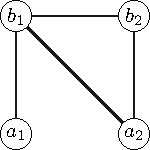
\includegraphics[scale=0.8]{H_4.pdf}} 
		\caption{Empacotamento de $P_6$ em $H_6$}
	\end{figure}
}

\frame{
	\frametitle{Escorpião}
	\begin{itemize}
		\setlength{\itemsep}{8pt}
		\item Um único vértice de grau maior a 2 (junção).
		\item No max. uma perna de comprimento maior a 2.
	\end{itemize}
	\vfill
	\begin{figure}
		\centering
		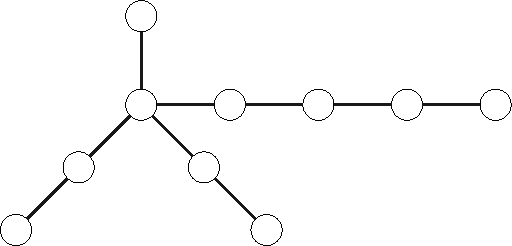
\includegraphics[scale=0.6]{scorpion.pdf}
		\caption{Escorpião de ordem 10.}
	\end{figure}
}

\setcounter{subfigure}{0}

\frame{
	\frametitle{Escorpião}
	\begin{figure}
		\centering
		\subfloat[$H_8$]{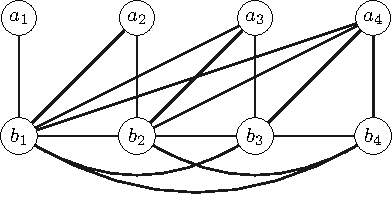
\includegraphics[scale=0.65]{H_8.pdf}}
		\\
		\subfloat{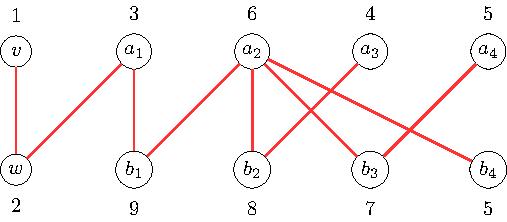
\includegraphics[scale=0.65]{scorpion-H10.pdf}}
		\caption{Empacotamento de escorpião no $H_{10}$}
	\end{figure}
}

\subsection{Limitando o tamanho da sequência}

\begin{frame}{\secname}
  \tableofcontents[currentsection,currentsubsection]
\end{frame}

\frame{
	\frametitle{Limitando el tamanho da sequência}
	Qual é o maior $s<n$ tal que $T_1, \ldots, T_s$ pode ser
	empacotado no $K_n$?
	\pause
	\vfill
	\begin{theorem}[Bollobás,1983]
		Se~$s \leq n / \sqrt{2} (\approx 0.7n)$, então $T_1, \ldots, T_s$ pode ser 
		empacotado no $K_n$.
	\end{theorem}
	\vfill
	\pause
	Dado um empacotamento de $T_{k+1}, \ldots, T_s$, como 
	empacotar $T_k$?
}

\frame{
	\frametitle{Limitando o tamanho da sequência}
	Dado um empacotamento de $T_{k+1}, \ldots, T_s$, como 
	empacotar $T_k$?
	\vfill
	\par
	Se $G = K_{n} - \cup_{i=k+1}^{n}{E(T_i)}$,
	\par
	\vfill
	\textbf{Ideia:} Encontrar $H \subseteq G$ tal que $\delta(H) \geq k - 1$.
	\pause
	\vfill
	\begin{figure}
		\centering
  		\subfloat{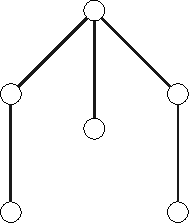
\includegraphics[scale=0.8]{T_6.pdf}}
		\qquad \qquad
		\subfloat{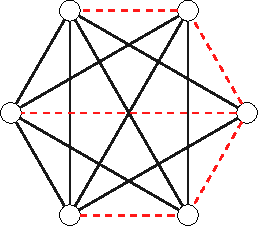
\includegraphics[scale=0.8	]{K_6.pdf}} 
	\end{figure}

}

\frame{
	\frametitle{Limitando o tamanho da sequência}
	\begin{proposition}
	Se $|E(G)| > \binom{k-1}{2} + (k-2)(n - k  + 1)$, então existe $H \subset G$
	tal que $\delta(H) \geq k-1$.
	\end{proposition}
	\vfill
	\par
	Se $s \leq n/\sqrt{2}$ e $G = K_n - \cup_{i=k+1}^{s}{E(T_i)}$
	\par
	\vfill
	$\Rightarrow$ $|E(G)| > \binom{k-1}{2} + (k-2)(n - k  + 1)$.
	\par
	\vfill
	Podemos melhorar o resultado?
	\pause 
	\vfill
	\begin{conjecture}[Erd\H{o}s \& Sós, 1963]
		Se $| E(G) | > (k-2)n / 2$, então $G$ contém qualquer árvore de ordem $k$.
	\end{conjecture}
}

\frame {
	\frametitle{Limitando o tamanho da sequência}
	\begin{conjecture}[Erd\H{o}s \& Sós, 1963]
		Se $| E(G) | > (k-2)n / 2$, então $G$ contém qualquer árvore de ordem $k$.
	\end{conjecture}
	\vfill
	Supondo a validez da conjectura anterior, obtemos que
	\vfill
	\par
	Se $s \leq \sqrt{3}n/2 \approx 0.86n$ $\Rightarrow$ podemos empacotar $T_1,\ldots,T_s$ no $K_n$.
}

\section{Variantes da conjectura de {\GL}}

\begin{frame}{\secname}
  \tableofcontents[currentsection]
\end{frame}

\frame{
	\frametitle{Variantes da conjectura}
	\begin{conjecture}[Hobbs et al., 1987]
		Uma sequência de árvores $T_1, \ldots, T_n$ 
		pode ser empacotada no $K_{n/2, n-1}$ se $n$ é par.
	\end{conjecture}
	\vfill
	\pause
	\begin{conjecture}[Gerbner et al., 2012]
		Uma sequência de árvores $T_1, \ldots, T_k$ pode ser empacotada 
		num grafo $k$-cromático.
	\end{conjecture}
	\vfill
	\pause
	\begin{conjecture}[Hollingsworth, 2013]
		Uma sequência de árvores balanceadas $\hat{T}_1, \ldots, \hat{T}_n$ 
		pode ser empacotada no $K_{n,n}$.
	\end{conjecture}
}

\subsection{Grafos bipartidos completos}

\begin{frame}{\secname}
  \tableofcontents[currentsection,currentsubsection]
\end{frame}

\frame{
	\frametitle{Resultados conhecidos}
		\begin{conjecture}[Hobbs et al., 1987]
		Uma sequência de árvores $T_1, \ldots, T_n$ 
		pode ser empacotada no $K_{n/2, n-1}$ se $n$ é par.
	\end{conjecture}
	\vfill
	\textbf{Restringimos a classe das árvores}
	\begin{itemize}
		\item Estrelas e caminhos. (Zaks \& Liu, 1976)
	\end{itemize}
	\vfill
	\pause
	\textbf{Limitando o tamanho da sequência}
	\par
	Podemos empacotar a sequência $T_1, \ldots, T_s$ no $K_n$
	\begin{itemize}
		\setlength{\itemsep}{8pt}
		\item Se $s \leq (\sqrt{13} - 3)n/2 \approx 0.3n$ (Caro \& Roditty, 1990).
		\item Se $s \leq \sqrt{5/8}n \approx 0.79n$ (Yuster, 1997).
	\end{itemize}
}

\subsection{Grafos $k$-cromáticos}
\frame{
	\frametitle{Empacotamento em grafos $k$-cromáticos}
		\begin{conjecture}[Gerbner et al., 2012]
		Uma sequência de árvores $T_1, \ldots, T_k$ pode ser empacotada 
		num grafo $k$-cromático.
	\end{conjecture}
	\pause
	\vfill
	A validez dessa afirmação implica a conjectura de {\GL}.
	\vfill
	\pause
	\begin{theorem}[Gerbner et al., 2012]
		Uma sequência de árvores $T_1, \ldots, T_k$ pode ser empacotada 
		num grafo $k$-cromático se no máximo 3 delas são diferentes de estrelas.
	\end{theorem}
}

\frame {
	\frametitle{Empacotamento em grafos $k$-cromáticos}
	\begin{theorem}[Gerbner et al., 2012]
		Uma sequência de árvores $T_1, \ldots, T_k$ pode ser empacotada 
		num grafo $k$-cromático se no máximo 3 delas são diferentes de estrelas.
	\end{theorem}
	\vfill
	Faremos a prova para quando no máximo $2$ das árvores não são estrelas.
	\par
	Suponha que 
	\vfill
	\begin{itemize}
		\item G é grafo $k$-cromático minimal ($\delta(G) \geq k-1$).
		\item Classes $C_1, \ldots, C_k$.
		\item $\forall v \in C_i$ existe $u \in C_{j}$ tq $uv \in E(G)$ $(j < i)$.
		\item $G_i$ é induzido por $C_k \cup C_{k-1} \cup \ldots \cup C_{k-i+1}$.
	\end{itemize}
}

\frame {
	\frametitle{Empacotamento em grafos $k$-cromáticos}
	Se $T_k$ ou $T_{k-1}$ é uma estrela, podemos fazer o 
	empacotamento como no caso do $K_n$.
	\vfill
	\pause 
	Suponha que $T_{k}$ e $T_{k-1}$ não são estrelas, e $T_{k-2}$ 
	e $T_{k-3}$ são estrelas.
	\vfill
	\par
	Sejam $T'_k = T_k - \{x_1,x_2\}$ e $T'_{k-1} = T_{k-1} - \{y_1,y_2\}$.
	\pause
	\par
	\vfill		
	\begin{figure}
		\centering
  		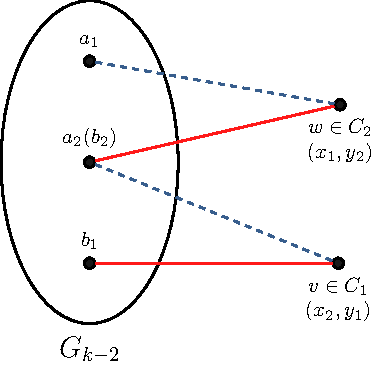
\includegraphics[scale=0.7]{figura4.pdf}
	\end{figure}
}

\frame {
	\frametitle{Empacotamento em grafos $k$-cromáticos}
	Para o caso em que $3$ árvores não são estrelas, a seguinte 
	asserção limita a estrutura de $T_k$.
	\vfill
	\begin{assertion}
		Se $T_k$ contém uma estrela pendurada de ordem~$s$ e
		$T_{k-s}$ é uma estrela, podemos empacotar $T_1,\ldots,T_k$,
		em $G$.
	\end{assertion}
	\pause
	\vfill
	Só falta considerar os casos onde $T_{k-2}$ ou
	$T_{k-3}$ não é uma estrela e $T_k$ tem estrelas penduradas de ordem 
	no max. 3. 
	\par
	\vfill	
	A prova se divide em muitos casos dependendo da estrutura de $T_k$,
	$T_{k-1}$ e $T_{k-2}$ ou $T_{k-3}$.
}

\section{Considerações finais}

\begin{frame}{\secname}
  \tableofcontents[currentsection,currentsubsection]
\end{frame}

\frame {
	\frametitle{Considerações finais}
	\begin{itemize}
		\item A técnica usada por Bollobás ajudou a obter  
		resultados em variantes da conjectura original.
		\vfill
		\item Quando restringimos as classes das árvores,
		as técnicas usadas não fornecem caminho claro para atacar
		a conjectura em sua forma mais geral.
	\end{itemize}
}

\frame{
	\begin{center}
	\huge
	Obrigado!!
	\vskip 5pt
	Gracias!!
	\end{center}
}

\end{document}
